% Options for packages loaded elsewhere
% Options for packages loaded elsewhere
\PassOptionsToPackage{unicode}{hyperref}
\PassOptionsToPackage{hyphens}{url}
%
\documentclass[
  ignorenonframetext,
  aspectratio=169,
]{beamer}
\newif\ifbibliography
\usepackage{pgfpages}
\setbeamertemplate{caption}[numbered]
\setbeamertemplate{caption label separator}{: }
\setbeamercolor{caption name}{fg=normal text.fg}
\beamertemplatenavigationsymbolsempty
% remove section numbering
\setbeamertemplate{part page}{
  \centering
  \begin{beamercolorbox}[sep=16pt,center]{part title}
    \usebeamerfont{part title}\insertpart\par
  \end{beamercolorbox}
}
\setbeamertemplate{section page}{
  \centering
  \begin{beamercolorbox}[sep=12pt,center]{section title}
    \usebeamerfont{section title}\insertsection\par
  \end{beamercolorbox}
}
\setbeamertemplate{subsection page}{
  \centering
  \begin{beamercolorbox}[sep=8pt,center]{subsection title}
    \usebeamerfont{subsection title}\insertsubsection\par
  \end{beamercolorbox}
}
% Prevent slide breaks in the middle of a paragraph
\widowpenalties 1 10000
\raggedbottom
\AtBeginPart{
  \frame{\partpage}
}
\AtBeginSection{
  \ifbibliography
  \else
    \frame{\sectionpage}
  \fi
}
\AtBeginSubsection{
  \frame{\subsectionpage}
}
\usepackage{iftex}
\ifPDFTeX
  \usepackage[T1]{fontenc}
  \usepackage[utf8]{inputenc}
  \usepackage{textcomp} % provide euro and other symbols
\else % if luatex or xetex
  \usepackage{unicode-math} % this also loads fontspec
  \defaultfontfeatures{Scale=MatchLowercase}
  \defaultfontfeatures[\rmfamily]{Ligatures=TeX,Scale=1}
\fi
\usepackage{lmodern}

\usetheme[]{Madrid}
\usecolortheme[]{default}
\usefonttheme[]{serif}
\ifPDFTeX\else
  % xetex/luatex font selection
\fi
% Use upquote if available, for straight quotes in verbatim environments
\IfFileExists{upquote.sty}{\usepackage{upquote}}{}
\IfFileExists{microtype.sty}{% use microtype if available
  \usepackage[]{microtype}
  \UseMicrotypeSet[protrusion]{basicmath} % disable protrusion for tt fonts
}{}
\makeatletter
\@ifundefined{KOMAClassName}{% if non-KOMA class
  \IfFileExists{parskip.sty}{%
    \usepackage{parskip}
  }{% else
    \setlength{\parindent}{0pt}
    \setlength{\parskip}{6pt plus 2pt minus 1pt}}
}{% if KOMA class
  \KOMAoptions{parskip=half}}
\makeatother


\usepackage{longtable,booktabs,array}
\newcounter{none} % for unnumbered tables
\usepackage{calc} % for calculating minipage widths
\usepackage{caption}
% Make caption package work with longtable
\makeatletter
\def\fnum@table{\tablename~\thetable}
\makeatother
\usepackage{graphicx}
\makeatletter
\newsavebox\pandoc@box
\newcommand*\pandocbounded[1]{% scales image to fit in text height/width
  \sbox\pandoc@box{#1}%
  \Gscale@div\@tempa{\textheight}{\dimexpr\ht\pandoc@box+\dp\pandoc@box\relax}%
  \Gscale@div\@tempb{\linewidth}{\wd\pandoc@box}%
  \ifdim\@tempb\p@<\@tempa\p@\let\@tempa\@tempb\fi% select the smaller of both
  \ifdim\@tempa\p@<\p@\scalebox{\@tempa}{\usebox\pandoc@box}%
  \else\usebox{\pandoc@box}%
  \fi%
}
% Set default figure placement to htbp
\def\fps@figure{htbp}
\makeatother





\setlength{\emergencystretch}{3em} % prevent overfull lines

\providecommand{\tightlist}{%
  \setlength{\itemsep}{0pt}\setlength{\parskip}{0pt}}



 


\makeatletter
\@ifpackageloaded{caption}{}{\usepackage{caption}}
\AtBeginDocument{%
\ifdefined\contentsname
  \renewcommand*\contentsname{Table of contents}
\else
  \newcommand\contentsname{Table of contents}
\fi
\ifdefined\listfigurename
  \renewcommand*\listfigurename{List of Figures}
\else
  \newcommand\listfigurename{List of Figures}
\fi
\ifdefined\listtablename
  \renewcommand*\listtablename{List of Tables}
\else
  \newcommand\listtablename{List of Tables}
\fi
\ifdefined\figurename
  \renewcommand*\figurename{Figure}
\else
  \newcommand\figurename{Figure}
\fi
\ifdefined\tablename
  \renewcommand*\tablename{Table}
\else
  \newcommand\tablename{Table}
\fi
}
\@ifpackageloaded{float}{}{\usepackage{float}}
\floatstyle{ruled}
\@ifundefined{c@chapter}{\newfloat{codelisting}{h}{lop}}{\newfloat{codelisting}{h}{lop}[chapter]}
\floatname{codelisting}{Listing}
\newcommand*\listoflistings{\listof{codelisting}{List of Listings}}
\makeatother
\makeatletter
\makeatother
\makeatletter
\@ifpackageloaded{caption}{}{\usepackage{caption}}
\@ifpackageloaded{subcaption}{}{\usepackage{subcaption}}
\makeatother

\usepackage{bookmark}
\IfFileExists{xurl.sty}{\usepackage{xurl}}{} % add URL line breaks if available
\urlstyle{same}
% fallback for those not using the hyperref driver hyperxmp:
\makeatletter
\@ifundefined{xmpquote}{\newcommand{\xmpquote}[1]{#1}}{}
\makeatother
\hypersetup{
  pdftitle={Project Title},
  pdfauthor={Jerry Jiang \textbar{} Mingzhe Li \textbar{} Yuk Shing Pang \textbar{} Jiayi Wu \textbar{} Group 202-A},
  hidelinks,
  pdfcreator={LaTeX via pandoc}}


\title{\texorpdfstring{Project Title}{Project Title}}
\subtitle{\texorpdfstring{Project subtitle (if
applicable)}{Project subtitle (if applicable)}}
\author{Jerry Jiang \textbar{} Mingzhe Li \textbar{} Yuk Shing Pang
\textbar{} Jiayi Wu \textbar{} Group 202-A}
\date{2026-11-19}

\begin{document}
\frame{\titlepage}


\begin{frame}{Introduction}
\protect\phantomsection\label{introduction}
\textbf{Overall Theme:} {[}State your unifying theme{]}

\textbf{Research Goal:} {[}What are you investigating?{]}

\textbf{Target Population:} {[}Who/what is being studied?{]}

\textbf{Audience:} {[}Who is this for?{]}
\end{frame}

\begin{frame}{Data Summary}
\protect\phantomsection\label{data-summary}
\textbf{Key Variables:}

\begin{itemize}
\tightlist
\item
  Variable 1: {[}Description{]}
\item
  Variable 2: {[}Description{]}
\end{itemize}

\textbf{Data Wrangling:}

\begin{itemize}
\tightlist
\item
  {[}Any transformations, new variables created{]}
\end{itemize}
\end{frame}

\begin{frame}{Question \#1: {[}Name - Question Statement{]}}
\protect\phantomsection\label{question-1-name---question-statement}
{[}Clear statement of the research question{]}
\end{frame}

\begin{frame}{Q1: Variables \& Approach}
\protect\phantomsection\label{q1-variables-approach}
\textbf{Variables used:}

\begin{itemize}
\tightlist
\item
  {[}List variables{]}
\end{itemize}

\textbf{New variables/groups defined:}

\begin{itemize}
\tightlist
\item
  {[}Any created variables{]}
\end{itemize}
\end{frame}

\begin{frame}{Q1: Visualization}
\protect\phantomsection\label{q1-visualization}
\begin{center}
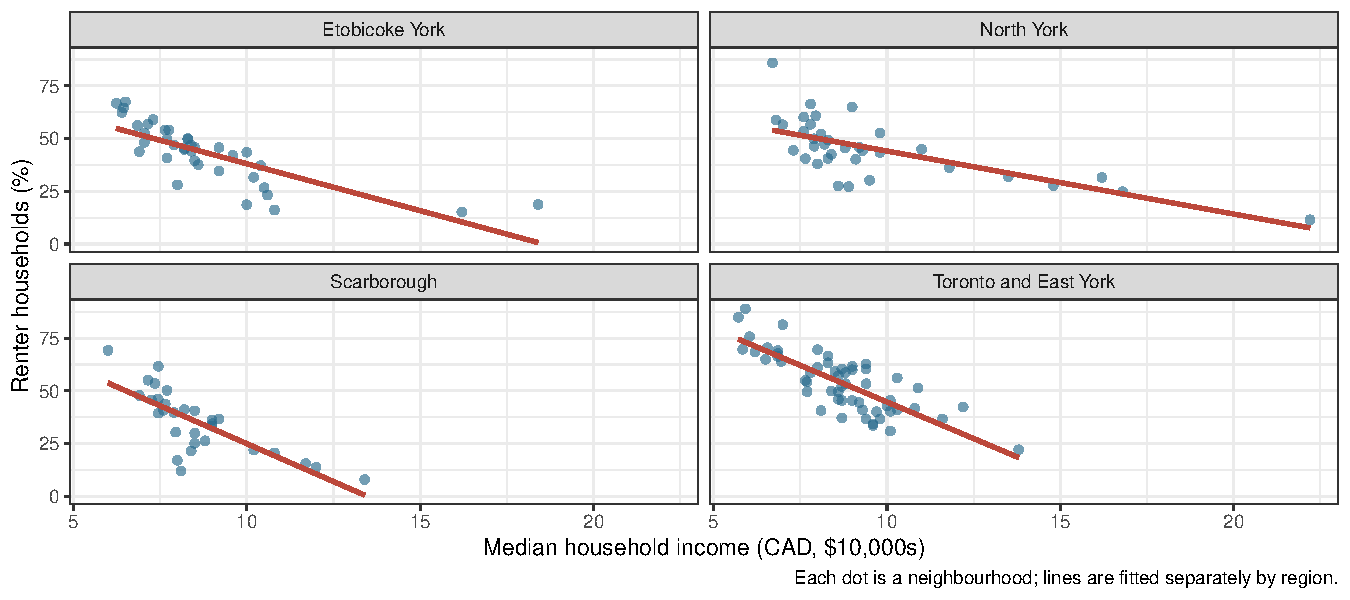
\includegraphics[width=0.8\linewidth,height=\textheight,keepaspectratio]{project-template_files/figure-beamer/q1-plot-1.pdf}
\end{center}
\end{frame}

\begin{frame}{Q1: Summary Table}
\protect\phantomsection\label{q1-summary-table}
\begin{longtable}[]{@{}lrrr@{}}
\caption{Comparison of Iris Species}\tabularnewline
\toprule\noalign{}
Species & Count & Avg Sepal Length & Avg Petal Length \\
\midrule\noalign{}
\endfirsthead
\toprule\noalign{}
Species & Count & Avg Sepal Length & Avg Petal Length \\
\midrule\noalign{}
\endhead
setosa & 50 & 5.0 & 1.5 \\
versicolor & 50 & 5.9 & 4.3 \\
virginica & 50 & 6.6 & 5.6 \\
\bottomrule\noalign{}
\end{longtable}

Insights for Q1
\end{frame}

\begin{frame}{Question \#2: {[}Name - Question Statement{]}}
\protect\phantomsection\label{question-2-name---question-statement}
{[}Repeat structure from Q1{]}
\end{frame}

\begin{frame}{Q2: Variables \& Approach}
\protect\phantomsection\label{q2-variables-approach}
\end{frame}

\begin{frame}{Q2: Visualization}
\protect\phantomsection\label{q2-visualization}
\end{frame}

\begin{frame}{Q2: Summary Table}
\protect\phantomsection\label{q2-summary-table}
\end{frame}

\begin{frame}{Question \#3: {[}Name - Question Statement{]}}
\protect\phantomsection\label{question-3-name---question-statement}
\end{frame}

\begin{frame}{Q3: Variables \& Approach}
\protect\phantomsection\label{q3-variables-approach}
\end{frame}

\begin{frame}{Q3: Visualization}
\protect\phantomsection\label{q3-visualization}
\end{frame}

\begin{frame}{Q3: Summary Table}
\protect\phantomsection\label{q3-summary-table}
\end{frame}

\begin{frame}{Question \#4: {[}Name - Question Statement{]} (if
applicable)}
\protect\phantomsection\label{question-4-name---question-statement-if-applicable}
\end{frame}

\begin{frame}{Q4: Variables \& Approach}
\protect\phantomsection\label{q4-variables-approach}
\end{frame}

\begin{frame}{Q4: Visualization}
\protect\phantomsection\label{q4-visualization}
\end{frame}

\begin{frame}{Q4: Summary Table}
\protect\phantomsection\label{q4-summary-table}
\end{frame}

\begin{frame}{Overall Limitations}
\protect\phantomsection\label{overall-limitations}
It is optional to include this as a stand-alone section at the end, you
could also choose to discuss this at the end of each research question

\textbf{Data Limitations:}

\begin{itemize}
\tightlist
\item
  {[}Limitation 1{]}
\item
  {[}Limitation 2{]}
\end{itemize}

\textbf{Future Directions:}

\begin{itemize}
\tightlist
\item
  {[}How these could be addressed{]}
\end{itemize}
\end{frame}

\begin{frame}{Overall Conclusion}
\protect\phantomsection\label{overall-conclusion}
\textbf{Key Findings:}

\begin{itemize}
\tightlist
\item
  {[}Finding 1 related to theme{]}
\item
  {[}Finding 2 related to theme{]}
\item
  {[}Finding 3 related to theme{]}
\end{itemize}

\textbf{Connection to Theme:}

{[}How findings relate back to unifying theme{]}
\end{frame}

\begin{frame}{References \& Acknowledgements (if applicable)}
\protect\phantomsection\label{references-acknowledgements-if-applicable}
\textbf{References:}

\begin{itemize}
\tightlist
\item
  {[}Citation 1, if applicable{]}
\end{itemize}

\textbf{Acknowledgements:}

\begin{itemize}
\tightlist
\item
  {[}Any acknowledgements, if applicable{]}
\end{itemize}
\end{frame}




\end{document}
